\documentclass[aspectratio=169, 10pt]{beamer}
\usetheme{metropolis}
\usepackage{amsmath, amssymb, booktabs, array, graphicx, tikz}
\usepackage[backend=biber,style=ieee,sorting=none]{biblatex}
\addbibresource{bibliography.bib}

\title{Predicting Psychiatric Illness Risk from\\Neuroimaging--Genetics Associations}
\subtitle{Master Thesis -- Progress Update}
\author{Leon Ackermann}
\date{March 12, 2026}

\begin{document}

\maketitle

% ============================================================
\section{Data}
% ============================================================

% ------ 1.1 Raw Data ------
\begin{frame}{Raw Participant-Level Data}
Two matrices share matched participant rows ($N_1 \ldots N_n$):

\medskip
\textbf{Structural MRI} ($n\times m$) \hfill \textbf{Genotype} ($n\times l$)

\[
\mathbf{X}_{\text{MRI}} =
\begin{pmatrix}
\text{MRI}_{1,1} & \cdots & \text{MRI}_{1,m}\\
\vdots & \ddots & \vdots\\
\text{MRI}_{n,1} & \cdots & \text{MRI}_{n,m}
\end{pmatrix}
\qquad
\mathbf{X}_{G} =
\begin{pmatrix}
G_{1,1} & \cdots & G_{1,l}\\
\vdots & \ddots & \vdots\\
G_{n,1} & \cdots & G_{n,l}
\end{pmatrix}
\]

\begin{itemize}
    \item $n$ = number of participants (European ancestry cohort)
    \item $m$ = MRI phenotypes (volume, area, thickness, intensity, contrast per brain region)
    \item $l$ = genotyped SNP variants
\end{itemize}
\end{frame}

% ------ 1.2 GWAS Transformation ------
\begin{frame}{GWAS Transformation}
For every SNP $i$ and MRI phenotype $j$, a GWAS collapses the $n$ participants into a single z-score:

\[
\text{GWAS}\!\bigl(\mathbf{X}_{G_{*,i}},\;\mathbf{X}_{\text{MRI}_{*,j}}\bigr)
\;\longrightarrow\; z_{i,j}
\]

Under a linear model for quantitative traits:
\[
y = G_{\text{MRI}_{*,j}}\,\beta^{G}_{i,j} + X\beta^{X} + e
\]

The z-score is
$\displaystyle z_{i,j} = \frac{\beta^{G}_{i,j}}{\mathrm{s.e.}(\beta^{G}_{i,j})}$.

\medskip
\begin{itemize}
    \item $\beta^{G}_{i,j}$: effect size of SNP $i$ on phenotype $j$
    \item $X,\beta^{X}$: covariates (age, sex, PCs\ldots)
    \item p-value: $\chi^{2} = \beta^{2}\cdot N$, then inverted
\end{itemize}
\end{frame}

% ------ 1.3 Final Dataset ------
\begin{frame}{Final Tabular ML Dataset (per illness)}
Rows = SNPs, features = MRI z-scores, target = illness z-score.

\[
\left[\;
\begin{array}{cccc|c}
z_{1,1} & z_{1,2} & \cdots & z_{1,m} & z_{\text{ill},1}\\
z_{2,1} & z_{2,2} & \cdots & z_{2,m} & z_{\text{ill},2}\\
\vdots  & \vdots  & \ddots & \vdots  & \vdots\\
z_{l,1} & z_{l,2} & \cdots & z_{l,m} & z_{\text{ill},l}
\end{array}
\;\right]
\begin{array}{l}
\leftarrow G_1\\
\leftarrow G_2\\
\vdots\\
\leftarrow G_l
\end{array}
\]

\begin{itemize}
    \item After clumping: $l \approx 3{,}500$ SNPs, $m \approx 1{,}000$ MRI features
    \item SCZ has highest predictive power (largest GWAS sample size)
    \item Negative median z-score is expected: allele ordering in GWAS is arbitrary
\end{itemize}
\end{frame}

% ------ 1.4 Clumping & LD ------
\begin{frame}{P-Value Clumping \& Linkage Disequilibrium}
\begin{itemize}
    \item Nearby nucleotides are correlated (LD) because recombination is less likely at short distances.
    \item $\mathrm{E}[\hat\beta_i] = \beta_i + \sum_{j\neq i} r_{ij}\beta_j$ (LD bias within a block).
    \item LD blocks are estimated in \textsc{PLINK}.
    \item \textbf{Clumping}: pick the lead SNP per LD block; remove all SNPs with $r^{2}$ above a threshold with the lead SNP.
    \item P-value threshold (e.g.\ $p < 10^{-3}$) controls how many SNPs survive $\Rightarrow$ dataset size vs.\ signal quality trade-off.
    \item Same SNP set is selected across illnesses $\Rightarrow$ cross-illness comparison is valid within European ancestry.
\end{itemize}
\end{frame}

% ============================================================
\section{Goal \& Task Formulation}
% ============================================================

\begin{frame}{ML Objective}
Learn a mapping:
\[
f(\mathbf{z}_i) \approx y_i,
\qquad
\mathbf{z}_i = [z_{i,1},\dots,z_{i,m}] \in \mathbb{R}^{m},
\quad
y_i \in \mathbb{R}
\]

\textbf{Two formulations:}
\begin{enumerate}
    \item \textbf{Regression}: predict the continuous illness z-score directly.\\
          $f\colon\mathbb{R}^{m}\to\mathbb{R}$
    \item \textbf{Binary classification}: threshold the z-score $\Rightarrow$ risk / no-risk label.\\
          Potentially more feasible given label distribution.
\end{enumerate}

\medskip
Both are instances of \emph{tabular machine learning}, which remains notoriously hard for unstructured feature sets \cite{kadraWelltunedSimpleNets, holzmullerBetterDefaultStrong2024}.
\end{frame}

% ============================================================
\section{Methods}
% ============================================================

\begin{frame}{Model Landscape}
\footnotesize
\begin{columns}[T,onlytextwidth]
\column{0.32\textwidth}
\begin{block}{Baselines}
\vspace{-2pt}
\begin{itemize}\setlength\itemsep{2pt}
    \item Linear Regression
    \item Lasso ($\ell_1$)
    \item Ridge ($\ell_2$)
    \item ElasticNet
\end{itemize}
\vspace{-2pt}
\end{block}

\column{0.32\textwidth}
\begin{block}{Boosted Trees}
\vspace{-2pt}
\begin{itemize}\setlength\itemsep{2pt}
    \item XGBoost \cite{chenXGBoostScalableTree2016}
    \item LightGBM \cite{keLightGBMHighlyEfficient}
    \item CatBoost \cite{prokhorenkovaCatBoostUnbiasedBoosting}
\end{itemize}
\vspace{-2pt}
\end{block}

\column{0.32\textwidth}
\begin{block}{Deep Learning}
\vspace{-2pt}
\begin{itemize}\setlength\itemsep{2pt}
    \item ResidualDNN \textit{(ours)}
    \item MLP + Reg.\ Cocktail \cite{kadraWelltunedSimpleNets}
    \item TabNet \cite{arikTabNetAttentiveInterpretable2021}
    \item TabPFNv2 \cite{hollmannAccuratePredictionsSmall2025}
\end{itemize}
\vspace{-2pt}
\end{block}
\end{columns}

\vspace{2em}
\begin{block}{Evaluation Protocol}
All models: 10 random seeds, 80/20 train/test.\quad Metrics: $R^2$, MSE (regression); AUC-ROC (classification).
\end{block}
\end{frame}

% ------ Baselines ------
\begin{frame}{Baseline Hyperparameters}
\footnotesize
\begin{table}
\centering
\begin{tabular}{@{}lll@{}}
\toprule
\textbf{Model} & \textbf{Key Hyperparameter} & \textbf{Value} \\
\midrule
Linear Regression & -- & OLS (no regularisation) \\
Lasso             & $\alpha$ & 0.0212 (via LassoCV) \\
Ridge             & $\alpha$ & 1000.0 (via RidgeCV) \\
ElasticNet        & $\alpha$, $\ell_1$-ratio & 0.0695, 0.1 \\
\midrule
XGBoost           & \texttt{n\_estimators}    & 200 \\
                  & \texttt{max\_depth}       & 3 \\
                  & \texttt{learning\_rate}   & 0.1 \\
                  & \texttt{subsample}        & 0.9 \\
                  & \texttt{colsample\_bytree} & 0.8 \\
\bottomrule
\end{tabular}
\end{table}

All models: 80/20 train/test split, 10 seeds (42--51).\\
Regularisation hyperparameters selected via cross-validated grid search.
\end{frame}

% ------ ResidualDNN ------
\begin{frame}{ResidualDNN Architecture}
\begin{columns}[T]
\column{0.55\textwidth}
\begin{itemize}\setlength\itemsep{3pt}
    \item Hidden dims: $[128, 128, 64, 64, 32, 32]$
    \item Paired into 3 \textbf{residual blocks} with skip connections
    \item Each block: Linear $\to$ ReLU $\to$ BatchNorm $\to$ Dropout(0.4) $\times 2$ Residual connection
    \item Optimiser: Adam, lr $= 10^{-5}$
    \item Gradient clipping at 1.0 to prevent exploding gradients
    \item Epochs: 300, batch size: 32
    \item Learning rate scheduler: Cosine Annealing with warm restarts (T\_0=15, T\_mult=2)
\end{itemize}

\column{0.4\textwidth}
\centering
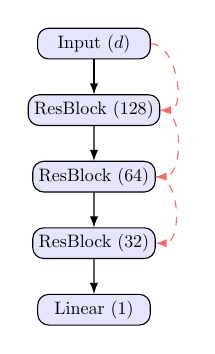
\begin{tikzpicture}[scale=0.65, every node/.style={scale=0.65},
    block/.style={draw, rounded corners, minimum width=2.2cm, minimum height=0.6cm, fill=blue!10}]
    \node[block] (in) at (0,0) {Input ($d$)};
    \node[block] (r1) at (0,-1.3) {ResBlock (128)};
    \node[block] (r2) at (0,-2.6) {ResBlock (64)};
    \node[block] (r3) at (0,-3.9) {ResBlock (32)};
    \node[block] (out) at (0,-5.2) {Linear (1)};
    \draw[-latex] (in) -- (r1);
    \draw[-latex] (r1) -- (r2);
    \draw[-latex] (r2) -- (r3);
    \draw[-latex] (r3) -- (out);
    % skip arrows
    \draw[-latex, dashed, red!60] (in.east) to[out=0,in=0] (r1.east);
    \draw[-latex, dashed, red!60] (r1.east) to[out=0,in=0] (r2.east);
    \draw[-latex, dashed, red!60] (r2.east) to[out=0,in=0] (r3.east);
\end{tikzpicture}
\end{columns}

\medskip
\footnotesize
\textbf{Outlook}: The \emph{Regularisation Cocktail} \cite{kadraWelltunedSimpleNets} adds weight decay, learning-rate warmup, mixup, cutout, and label smoothing on top of a plain MLP---further avenues for improvement.
\end{frame}

% ============================================================
\section{Results}
% ============================================================

\begin{frame}{Results -- Schizophrenia (SCZ)}
\footnotesize
\begin{table}
\centering
\begin{tabular}{@{}lcc@{}}
\toprule
\textbf{Model} & \textbf{Mean $R^{2}$} & \textbf{Mean MSE} \\
\midrule
Residual DNN      & \textbf{0.409} & \textbf{13.10} \\
ElasticNet        & 0.393          & 13.47 \\
Ridge             & 0.385          & 13.64 \\
Lasso             & 0.382          & 13.70 \\
XGBoost           & 0.349          & 14.45 \\
Linear Regression & 0.258          & 16.47 \\
\bottomrule
\end{tabular}
\caption{Aggregated over 10 seeds (42--51), 80/20 split.}
\end{table}

\begin{itemize}
    \item Regularised linear models outperform plain OLS substantially ($+0.12$ $R^{2}$).
    \item XGBoost under-performs linear baselines---likely due to limited sample size ($\sim$3.5k).
    \item ResidualDNN achieves the best $R^{2}$ so far, suggesting non-linear signal is present.
\end{itemize}
\end{frame}

% ============================================================
\section{Next Steps}
% ============================================================

\begin{frame}{Next Steps}
\begin{enumerate}\setlength\itemsep{6pt}
    \item \textbf{Regularisation Cocktail MLP}\\
          Systematically search weight decay, mixup, cutout, learning-rate schedules, and label smoothing \cite{kadraWelltunedSimpleNets}.

    \item \textbf{Pre-trained TabTransformer (TabPFN-style)}\\
          Pre-train a transformer on MRI--GWAS data across multiple illnesses, then fine-tune on target illness. Inspired by \cite{hollmannAccuratePredictionsSmall2025}.

    \item \textbf{Graph Neural Network}\\
          Treat brain regions as nodes with MRI features; edge definition TBD (spatial adjacency, functional connectivity, or learned).

    \item \textbf{Classification formulation}\\
          Threshold z-score into binary risk labels; evaluate with AUC-ROC alongside $R^{2}$.


\end{enumerate}
\end{frame}

% ============================================================
% References
% ============================================================

\begin{frame}[allowframebreaks]{References}
\footnotesize
\printbibliography
\end{frame}

\end{document}
